\documentclass[11pt]{article}
\usepackage[review]{acl}
\usepackage{times}
\usepackage{latexsym}
\usepackage[T1]{fontenc}
\usepackage[utf8]{inputenc}
\usepackage{microtype}
\usepackage{inconsolata}
\usepackage{booktabs}
\usepackage{multirow}
\usepackage{graphicx}
\usepackage{amsmath,amssymb}
\usepackage{tikz}
\usetikzlibrary{shapes.geometric, arrows.meta, positioning, fit, backgrounds, calc}
\usepackage{pgfplots}
\pgfplotsset{compat=1.18}
\usepackage{xcolor}
\usepackage{array}
\usepackage{makecell}
\usepackage{footnote}
\usepackage{url}
\usepackage{subcaption}

%% Color palette
\definecolor{c1}{RGB}{31,119,180}   % blue
\definecolor{c2}{RGB}{255,127,14}   % orange
\definecolor{c3}{RGB}{44,160,44}    % green
\definecolor{c4}{RGB}{214,39,40}    % red
\definecolor{c5}{RGB}{148,103,189}  % purple
\definecolor{lightgray}{RGB}{240,240,240}

\title{From Retrieval to Reasoning:\\
A Survey of Knowledge Graph-Enhanced\\
Retrieval-Augmented Generation}

\author{
  Anonymous ACL Submission
}

\begin{document}
\maketitle

%% ============================================================
\begin{abstract}
Retrieval-Augmented Generation (RAG) has emerged as the de facto paradigm for grounding large language model (LLM) outputs in external knowledge. However, standard RAG systems—which retrieve flat text chunks—struggle with multi-hop reasoning, relational inference, and global corpus-level understanding. Knowledge graphs (KGs) offer a structured alternative: their explicit entity-relation representation naturally supports compositional reasoning. This survey provides a comprehensive review of \emph{Knowledge Graph-Enhanced RAG} (GraphRAG), a rapidly growing field at the intersection of KG reasoning and LLM generation. We propose a two-dimensional taxonomy that distinguishes methods by \emph{KG source} (pre-built symbolic KGs vs.\ corpus-induced graphs) and \emph{retrieval mechanism} (traversal, subgraph retrieval, and graph propagation). We systematically review over 25 representative methods across both dimensions, analyze state-of-the-art results on six standard benchmarks, and identify seven open research challenges. Our survey aims to serve as a structured entry point and research roadmap for the growing community working at the intersection of structured knowledge and language models.
\end{abstract}

%% ============================================================
\section{Introduction}
\label{sec:intro}

Large language models (LLMs) have demonstrated remarkable abilities in language understanding and generation \cite{lewis2020rag}. Yet their closed-book parametric knowledge is static, opaque, and prone to hallucination on knowledge-intensive tasks. Retrieval-Augmented Generation (RAG) \cite{lewis2020rag,guu2020realm} addresses this by conditioning LLM generation on dynamically retrieved evidence, yielding systems that are more factual, up-to-date, and verifiable.

Despite its success, \emph{flat} RAG—retrieving and concatenating text passages—faces fundamental limitations for complex reasoning. First, \textbf{multi-hop inference} requires chaining evidence across multiple passages, but flat retrieval systems have no mechanism to follow relational chains. Second, \textbf{compositional queries} such as ``Who directed the film starring the actor who won the 2019 Academy Award?'' require structured understanding of entity relationships, not mere lexical overlap. Third, \textbf{global analysis}—``What are the main themes across this corpus?''—cannot be answered by any individual retrieved chunk.

Knowledge Graphs (KGs) naturally address these gaps. A KG encodes world knowledge as a set of typed triples $(h, r, t)$, where entities $h, t$ are connected by a relation $r$. This structure explicitly represents the multi-hop connections that flat RAG must infer, enables compositional query planning along relation paths, and supports global summarization through hierarchical community structure.

\textbf{Knowledge Graph-Enhanced RAG} (GraphRAG) is the umbrella term for methods that combine the factual precision of KGs with the reasoning fluency of LLMs. The field has grown rapidly, producing systems ranging from simple KG-prompting \cite{baek2023kaping} to iterative LLM-KG traversal \cite{sun2024tog}, learned subgraph retrieval \cite{wang2025subgraphrag}, and community-indexed corpus analysis \cite{edge2024graphrag}.

\textbf{Contributions.} This survey makes the following contributions:
\begin{enumerate}
\item A two-dimensional \textbf{taxonomy} that systematically organizes GraphRAG methods by KG source and retrieval mechanism (\S\ref{sec:taxonomy}).
\item A thorough \textbf{method review} covering over 25 representative systems with analysis of their design choices and trade-offs (\S\ref{sec:prebuilt}--\S\ref{sec:corpus}).
\item A structured \textbf{benchmark analysis} with state-of-the-art results across six benchmarks (\S\ref{sec:benchmarks}).
\item \textbf{Cross-cutting analysis} of efficiency, supervision quality, and scalability (\S\ref{sec:analysis}).
\item A set of \textbf{open research challenges} to guide future work (\S\ref{sec:challenges}).
\end{enumerate}

%% ============================================================
\section{Background}
\label{sec:background}

\subsection{The RAG Paradigm}

A standard RAG system comprises three components: (1) an \emph{indexer} that encodes a corpus into a searchable index; (2) a \emph{retriever} $f_R(q) \rightarrow \mathcal{D}$ that maps a query $q$ to a set of evidence passages $\mathcal{D}$; and (3) a \emph{generator} that produces the final answer conditioned on $q$ and $\mathcal{D}$.

Early work established the foundational retrieve-then-generate pipeline \cite{lewis2020rag,guu2020realm}. Subsequent methods explored multi-document fusion \cite{izacard2021fid}, retrieval-augmented pre-training at scale \cite{borgeaud2022retro,izacard2022atlas}, and adaptive retrieval strategies \cite{asai2024selfrag,jeong2024adaptiverag}. Surveys by \citet{gao2023ragsurvey} and \citet{gao2024modularrag} provide comprehensive treatments of the broader RAG landscape.

\subsection{Knowledge Graphs in NLP}

A Knowledge Graph $\mathcal{G} = (\mathcal{E}, \mathcal{R}, \mathcal{T})$ consists of entities $\mathcal{E}$, relation types $\mathcal{R}$, and a set of triples $\mathcal{T} \subseteq \mathcal{E} \times \mathcal{R} \times \mathcal{E}$. Large-scale KGs include Freebase (used in KGQA benchmarks), Wikidata, and domain-specific KGs. They have long been used for question answering via semantic parsing (SP-KGQA) and embedding-based methods \cite{saxena2020embedkgqa,jiang2023unikgqa}. The advent of LLMs opened a new paradigm: rather than reasoning over KGs directly, LLMs can be augmented with KG-derived evidence, combining the structure of KGs with the fluency of neural generation \cite{pan2024kgllmsurvey}.

%% ============================================================
\section{Taxonomy of GraphRAG Methods}
\label{sec:taxonomy}

We organize GraphRAG methods along two orthogonal dimensions:

\paragraph{Dimension 1: KG Source.}
\begin{itemize}
  \item \textbf{Pre-built KGs} (e.g., Freebase, WikiMovies): curated, high-precision, but domain-restricted and potentially incomplete.
  \item \textbf{Corpus-induced KGs}: extracted on-the-fly from the target document collection via LLM-based entity/relation extraction. More flexible but noisier.
\end{itemize}

\paragraph{Dimension 2: Retrieval Mechanism.}
\begin{itemize}
  \item \textbf{KG-prompting}: directly inject retrieved triples as textual context.
  \item \textbf{Iterative traversal}: an LLM agent walks the KG step by step.
  \item \textbf{Plan-then-retrieve}: generate a relation path plan first; retrieve matching KG paths.
  \item \textbf{Subgraph retrieval}: train a scorer to retrieve a relevant subgraph in one shot.
  \item \textbf{Graph propagation}: spread query relevance through graph topology (e.g., PageRank).
  \item \textbf{Community summarization}: detect communities in the graph; summarize them for global queries.
\end{itemize}

Figure~\ref{fig:taxonomy} illustrates this taxonomy. Table~\ref{tab:methods} summarizes key properties of representative methods.

\begin{figure*}[t]
\centering
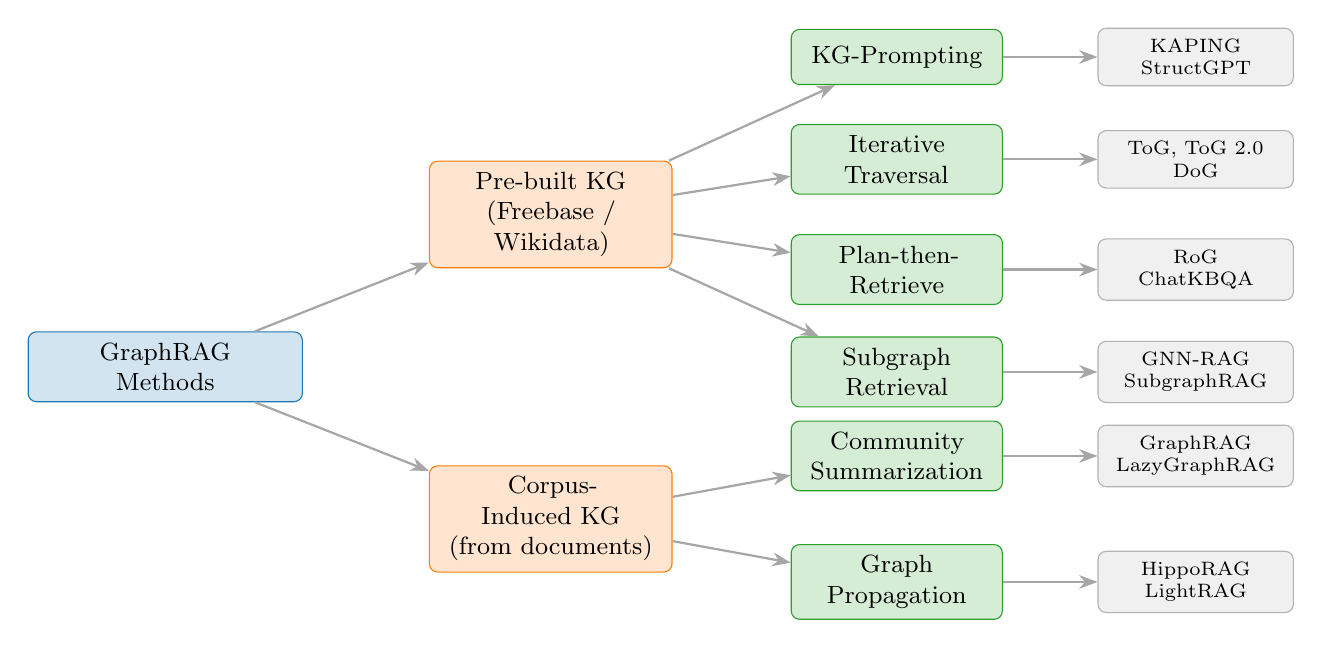
\begin{tikzpicture}[
  node distance=0.5cm and 1.2cm,
  every node/.style={font=\small},
  box/.style={rectangle, rounded corners=3pt, draw, align=center, minimum height=0.7cm, inner sep=4pt},
  rootbox/.style={box, fill=c1!20, draw=c1, text width=3.2cm},
  dim1/.style={box, fill=c2!20, draw=c2, text width=2.8cm},
  dim2/.style={box, fill=c3!20, draw=c3, text width=2.4cm},
  leaf/.style={box, fill=lightgray, draw=gray!60, text width=2.2cm, font=\scriptsize},
  arr/.style={-Stealth, gray!70, thick},
]
%% Root
\node[rootbox] (root) {GraphRAG\\Methods};

%% KG Source dimension
\node[dim1, above right=0.8cm and 1.6cm of root] (prebuilt) {Pre-built KG\\(Freebase / Wikidata)};
\node[dim1, below right=0.8cm and 1.6cm of root] (corpus) {Corpus-Induced KG\\(from documents)};

\draw[arr] (root) -- (prebuilt);
\draw[arr] (root) -- (corpus);

%% Pre-built subtypes
\node[dim2, right=1.5cm of prebuilt, yshift=2.0cm]  (prompt)   {KG-Prompting};
\node[dim2, right=1.5cm of prebuilt, yshift=0.7cm]  (traversal){Iterative\\Traversal};
\node[dim2, right=1.5cm of prebuilt, yshift=-0.7cm] (plan)     {Plan-then-\\Retrieve};
\node[dim2, right=1.5cm of prebuilt, yshift=-2.0cm] (subgraph) {Subgraph\\Retrieval};

\draw[arr] (prebuilt) -- (prompt);
\draw[arr] (prebuilt) -- (traversal);
\draw[arr] (prebuilt) -- (plan);
\draw[arr] (prebuilt) -- (subgraph);

%% Corpus subtypes
\node[dim2, right=1.5cm of corpus, yshift=0.8cm]  (community) {Community\\Summarization};
\node[dim2, right=1.5cm of corpus, yshift=-0.8cm] (propagate) {Graph\\Propagation};

\draw[arr] (corpus) -- (community);
\draw[arr] (corpus) -- (propagate);

%% Leaves — pre-built
\node[leaf, right=1.2cm of prompt]    (l1) {KAPING\\StructGPT};
\node[leaf, right=1.2cm of traversal] (l2) {ToG, ToG~2.0\\DoG};
\node[leaf, right=1.2cm of plan]      (l3) {RoG\\ChatKBQA};
\node[leaf, right=1.2cm of subgraph]  (l4) {GNN-RAG\\SubgraphRAG};

\draw[arr] (prompt)    -- (l1);
\draw[arr] (traversal) -- (l2);
\draw[arr] (plan)      -- (l3);
\draw[arr] (subgraph)  -- (l4);

%% Leaves — corpus
\node[leaf, right=1.2cm of community] (l5) {GraphRAG\\LazyGraphRAG};
\node[leaf, right=1.2cm of propagate] (l6) {HippoRAG\\LightRAG};

\draw[arr] (community) -- (l5);
\draw[arr] (propagate) -- (l6);

\end{tikzpicture}
\caption{Two-dimensional taxonomy of GraphRAG methods organized by KG source (pre-built vs.\ corpus-induced) and retrieval mechanism.}
\label{fig:taxonomy}
\end{figure*}

%% ============================================================
\section{Pre-built KG GraphRAG}
\label{sec:prebuilt}

\subsection{KG-Prompting}
\label{sec:prompting}

The simplest GraphRAG paradigm injects KG triples directly into the LLM prompt as supplementary textual context. \textbf{KAPING} \cite{baek2023kaping} retrieves facts from a KG that are semantically similar to the query entities and concatenates them as soft prefix context. The approach requires no fine-tuning and generalizes across LLMs. \textbf{StructGPT} \cite{jiang2023structgpt} generalizes this idea to arbitrary structured data (KGs, tables, databases) via an Iterative Reading-then-Reasoning (IRR) framework in which an LLM invokes typed data-access functions iteratively, accumulating structured evidence before generating the final answer. These methods establish important baselines: they demonstrate that even naive KG injection improves factual accuracy but suffer from noise when retrieved triples include irrelevant facts.

\subsection{Iterative LLM-KG Traversal}
\label{sec:traversal}

Rather than pre-fetching context, iterative traversal methods allow an LLM to \emph{explore} the KG dynamically. \textbf{Think-on-Graph (ToG)} \cite{sun2024tog} treats the LLM as a beam-search agent that iteratively: (1) selects which relations to follow from the current entity frontier, (2) expands the frontier, (3) prunes irrelevant entities, and (4) generates the final answer when sufficient evidence is accumulated. ToG can handle arbitrary hop-depth queries and produces interpretable reasoning chains aligned with KG structure. \textbf{ToG 2.0} \cite{ma2025tog2} extends this with \emph{deep thinking}: a chain-of-thought reasoning pass within each beam step that uses LLM self-consistency to prune impossible paths before expansion, reducing both latency and hallucination. \textbf{Debate on Graph (DoG)} \cite{ma2025dog} introduces a multi-agent extension: a proponent and opponent LLM explore the KG independently and then debate their retrieved evidence under a judge LLM, with disagreement driving targeted re-retrieval. On WebQSP, DoG achieves 91.0 Hits@1 with GPT-4, the highest reported result with a proprietary model.

Despite strong accuracy, iterative traversal methods are expensive: each reasoning step incurs one or more LLM calls, making latency proportional to query complexity and beam width.

\subsection{Plan-then-Retrieve}
\label{sec:plan}

Plan-then-retrieve methods decouple the reasoning plan from the evidence retrieval step. \textbf{RoG} \cite{luo2024rog} fine-tunes an LLM to first generate a \emph{relation path} (e.g., \texttt{born\_in}$\rightarrow$\texttt{located\_in}) as a high-level plan, then retrieves all KG paths matching this plan, and finally generates the answer over the retrieved paths. The plan imposes a strong structural prior on retrieval, reducing noise from unrelated subgraphs. \textbf{ChatKBQA} \cite{luo2024chatkbqa} fine-tunes an LLM to generate SPARQL-like S-expressions (logical forms), then applies entity linking and relation retrieval to ground the generated expression onto the actual KG. A post-hoc disambiguation module handles entity name ambiguity common in large KGs. Both methods achieve strong performance on WebQSP and CWQ but require fine-tuning on KG-specific supervision, limiting cross-domain applicability.

\subsection{Subgraph Retrieval}
\label{sec:subgraph}

Subgraph retrieval methods aim to extract a compact, relevant subgraph in a single forward pass—avoiding iterative LLM calls while providing richer context than individual triples.

\textbf{UniKGQA} \cite{jiang2023unikgqa} unifies retrieval and reasoning in a single shared-parameter model. A retrieval module scores candidate relation paths starting from topic entities; a reasoning module aggregates the retrieved triples to produce the final answer distribution. Joint training allows the retrieval and reasoning components to co-adapt.

\textbf{GNN-RAG} \cite{mavromatis2024gnnrag} takes a hybrid approach: first runs a GNN (LHNN) trained on KGQA to predict answer entities, then extracts shortest KG paths between question entities and predicted answers as the LLM's retrieval context. The GNN provides structural inductive bias unavailable to pure LLM-based methods. GNN-RAG further incorporates text-passage retrieval augmentation (RA), achieving 87.0 Hits@1 on WebQSP with LLaMA-2-7B.

\textbf{SubgraphRAG} \cite{wang2025subgraphrag} takes a different approach: a lightweight MLP scores \emph{each triple independently} using concatenated semantic features $[q, h, r, t]$ supplemented by Degree-based Distinguishing Embeddings (DDE)—a non-parametric structural encoding derived by mean-aggregating neighbor distances from topic entities. Trained with binary cross-entropy on shortest-path weak labels, the retriever selects the top-$K$ triples ($K{=}100$) as flat context for an LLM. The key finding is that this simple design, when paired with a sufficiently capable LLM (GPT-4o-mini), matches or exceeds iterative traversal methods at a fraction of the inference cost: 87.4 Hits@1 and 78.3 F1 on WebQSP. The paper's central thesis—that the LLM backbone quality dominates retrieval method complexity—is supported by ablations across five LLMs.

\textbf{G-Retriever} \cite{he2024gretriever} addresses a complementary setting: QA over \emph{text-attributed graphs} where nodes and edges carry rich textual descriptions. A Prize-Collecting Steiner Tree (PCST) algorithm extracts a minimal connected subgraph linking query-relevant nodes. The subgraph is encoded by a graph transformer (GraphGPS) and injected into an LLM via soft prompting, enabling multi-hop reasoning over graphs that are neither pure symbolic KGs nor plain text.

\subsection{Reward-Optimized Retrieval}
\label{sec:reward}

Recent work applies reinforcement learning to directly optimize retrieval toward downstream QA reward. \textbf{RoE} \cite{han2025roe} fine-tunes LLaMA-3.1-8B to generate action sequences (explore entity, follow relation, verify answer) as structured exploration traces, trained with answer-match reward via PPO. \textbf{RPO-RAG} \cite{um2026rporag} employs relation-aware preference optimization (DPO-style) to teach the LLM to both retrieve better relation paths and reason over them jointly, achieving 89.9 Hits@1 and 81.3 F1 on WebQSP—the current best result with an open-source LLM. These methods represent the frontier of the field, suggesting that end-to-end reward-guided training of the full retrieve-and-reason pipeline will be a dominant direction going forward.

%% ============================================================
\section{Corpus-Induced KG GraphRAG}
\label{sec:corpus}

While pre-built KG methods require curated symbolic KGs (Freebase, Wikidata), corpus-induced GraphRAG methods build their own graph structure from the target document collection using LLM-based extraction. This makes them applicable to arbitrary private or domain-specific corpora.

\subsection{Community-based Summarization}
\label{sec:community}

\textbf{Microsoft GraphRAG} \cite{edge2024graphrag} is the seminal work in corpus-induced GraphRAG. The indexing pipeline: (1) applies an LLM to extract entity and relation triples from every text chunk; (2) builds a graph over these entities; (3) applies hierarchical Leiden community detection to partition the graph into nested communities; (4) generates LLM summaries for each community at multiple resolution levels. Query time uses two modes: \emph{local search} follows entity-centric subgraphs to answer factoid queries, while \emph{global search} aggregates community summaries via a map-reduce LLM pipeline to answer corpus-level analytical queries such as ``What are the dominant themes?'' Empirically, global GraphRAG substantially outperforms standard RAG on abstract and analytical queries \cite{edge2024graphrag}. The primary limitation is indexing cost: LLM calls for extraction and summarization make full indexing expensive for large corpora. \textbf{LazyGraphRAG} \cite{edge2024graphrag} addresses this by deferring community summarization to query time—building only a lightweight entity extraction index upfront and summarizing only the communities relevant to a given query, reducing indexing cost by an order of magnitude.

\subsection{Graph Propagation}
\label{sec:propagation}

\textbf{HippoRAG} \cite{gutierrez2024hipporag} draws inspiration from the hippocampal memory model in cognitive neuroscience. An LLM extracts a schematic KG from the document corpus; query-relevant entities are identified by dense retrieval, and then Personalized PageRank (PPR) seeded from these entities propagates relevance through the graph. The PPR scores rank passages for final retrieval. By capturing multi-hop graph connectivity, HippoRAG retrieves associatively linked evidence that dense retrieval misses, outperforming IRCoT-style iterative retrieval \cite{trivedi2023ircot} on multi-hop QA benchmarks at lower latency.

\textbf{LightRAG} \cite{guo2024lightrag} builds a dual-level index: a fine-grained entity-level graph and a coarse-grained relation-level hypergraph. It supports both specific (low-level) and abstract (high-level) queries through a unified retrieval interface, and supports incremental graph updates without full re-indexing—addressing a key practical limitation of GraphRAG for dynamic document corpora.

%% ============================================================
\section{Benchmarks and Evaluation}
\label{sec:benchmarks}

\subsection{Datasets}

Table~\ref{tab:datasets} summarizes the standard benchmarks. \textbf{WebQSP} \cite{yih2016webqsp} and \textbf{CWQ} \cite{talmor2018cwq} are the primary KGQA benchmarks over Freebase, covering 1--2 and 2--4 hop questions respectively. \textbf{MetaQA-3hop} \cite{zhang2018metaqa} is a 3-hop chain benchmark over the WikiMovies KG, now considered saturated for trained methods (TransferNet achieves 100\% Hits@1) but useful as a zero-shot transfer target. \textbf{HotpotQA} \cite{yang2018hotpotqa}, \textbf{2WikiMultiHopQA} \cite{ho2020wikimultihop}, and \textbf{MuSiQue} \cite{trivedi2022musique} form the standard open-domain multi-hop QA suite over Wikipedia text, where the KG is implicitly encoded in documents rather than provided as a structured resource.

\begin{table}[t]
\centering
\small
\caption{Benchmark datasets. \textit{Hops}: reasoning depth. \textit{KG}: structured KG provided.}
\label{tab:datasets}
\setlength{\tabcolsep}{4pt}
\begin{tabular}{lcccc}
\toprule
\textbf{Dataset} & \textbf{Hops} & \textbf{KG} & \textbf{Test Size} & \textbf{Metric} \\
\midrule
WebQSP  & 1--2 & \checkmark & 1,628   & Hits@1, F1 \\
CWQ     & 2--4 & \checkmark & 3,519   & Hits@1, F1 \\
MetaQA-3hop & 3 & \checkmark & $\sim$14K & Hits@1 \\
HotpotQA    & 2   & --         & 7,405   & Joint F1 \\
2WikiMultiHop & 2--4 & --      & 12,576  & F1, EM \\
MuSiQue     & 2--4 & --       & 2,417   & F1, EM \\
\bottomrule
\end{tabular}
\end{table}

\subsection{State-of-the-Art Results}

Table~\ref{tab:sota} reports state-of-the-art results on the two primary KGQA benchmarks. Several trends are noteworthy. First, LLM-augmented KG methods have dramatically outpaced traditional GNN-based KGQA (e.g., NSM, UniKGQA) since 2023, widening the gap from $\sim$77 to $\sim$91 Hits@1 on WebQSP. Second, the LLM backbone quality has an outsized effect on final performance; SubgraphRAG with GPT-4o-mini (87.4) outperforms the same retriever with LLaMA-3.1-8B ($\sim$72) by a large margin. Third, reward-optimized methods (RoE, RPO-RAG) trained with small LLMs are rapidly closing the gap with GPT-4-based systems, suggesting that the bottleneck is increasingly the retrieval-reasoning training signal rather than raw LLM capability.

\begin{table*}[t]
\centering
\small
\caption{State-of-the-art results on WebQSP and CWQ. \textbf{Bold}: best per LLM tier.
``Open'' = open-source LLM ($\leq$13B unless noted). ``Prop.'' = proprietary LLM.
``FT'' = fine-tuned. ``--'' = not reported.}
\label{tab:sota}
\setlength{\tabcolsep}{5pt}
\begin{tabular}{llccccc}
\toprule
\multirow{2}{*}{\textbf{Method}} & \multirow{2}{*}{\textbf{Backbone}} &
\multicolumn{2}{c}{\textbf{WebQSP}} & \multicolumn{2}{c}{\textbf{CWQ}} &
\multirow{2}{*}{\textbf{Tier}} \\
\cmidrule(lr){3-4}\cmidrule(lr){5-6}
& & \textit{Hits@1} & \textit{F1} & \textit{Hits@1} & \textit{F1} & \\
\midrule
\multicolumn{7}{l}{\textit{GNN / Embedding baselines (no LLM)}} \\
NSM          & --                    & 68.7 & 62.8 & 47.6 & 42.4 & -- \\
UniKGQA      & --                    & 77.2 & 72.2 & 51.2 & 49.1 & -- \\
ReaRev       & --                    & 77.5 & 72.8 & 53.3 & 49.7 & -- \\
\midrule
\multicolumn{7}{l}{\textit{LLM-augmented methods}} \\
KAPING       & GPT-3.5               & 52.4 & --   & 31.2 & --   & Prop. \\
ToG          & ChatGPT               & 76.2 & --   & 58.9 & --   & Prop. \\
RoG          & LLaMA-2-7B (FT)       & 85.7 & 70.8 & 62.6 & 56.2 & Open \\
GNN-RAG      & LLaMA-2-7B            & 85.7 & 71.3 & 66.8 & 59.4 & Open \\
GNN-RAG+RA   & LLaMA-2-7B            & 87.0 & 73.5 & 68.7 & 60.4 & Open \\
ChatKBQA     & LLaMA-2-13B (FT)      & 87.9 & 75.1 & 68.5 & --   & Open \\
SubgraphRAG  & GPT-4o-mini           & 87.4 & 78.3 & 65.0 & 58.4 & Prop. \\
SubgraphRAG  & GPT-4o                & 86.4 & 77.6 & \textbf{68.9} & \textbf{66.0} & Prop. \\
ToG          & GPT-4                 & 82.6 & --   & 67.6 & --   & Prop. \\
DoG          & GPT-3.5               & 88.6 & --   & 58.2 & --   & Prop. \\
\textbf{DoG} & GPT-4                 & \textbf{91.0} & -- & 56.0 & -- & Prop. \\
\midrule
\multicolumn{7}{l}{\textit{RL / preference-optimized (small LLMs)}} \\
RoE          & LLaMA-3.1-8B (FT)     & 89.1 & 74.8 & 66.5 & 53.2 & Open \\
\textbf{RPO-RAG} & LLaMA-3.1-8B (FT) & \textbf{89.9} & \textbf{81.3} & \textbf{72.3} & \textbf{64.5} & Open \\
\bottomrule
\end{tabular}
\end{table*}

\subsection{Evaluation Gaps}

Several evaluation challenges complicate fair comparison. (1) \emph{Metric inconsistency}: Hits@1 and F1 measure different properties (recall vs.\ token overlap) and are not directly comparable across papers. (2) \emph{Entity linking dependency}: most methods rely on gold topic entities provided by the benchmark, which over-estimates real-world performance. (3) \emph{KG version mismatch}: Freebase has multiple versions; triple coverage varies significantly across subsets, inflating some method's scores. (4) \emph{Benchmark saturation}: MetaQA-3hop (100\% since 2021) and partially WebQSP provide limited headroom for differentiation. For multi-hop text RAG benchmarks (HotpotQA, MuSiQue), LLM-era papers typically report Answer F1 in open-domain settings, which is not comparable to the Joint F1 on the official leaderboard, making cross-paper comparison unreliable.

%% ============================================================
\section{Cross-Cutting Analysis}
\label{sec:analysis}

\subsection{Efficiency vs.\ Accuracy Trade-off}

Figure~\ref{fig:efficiency} illustrates the qualitative efficiency-accuracy trade-off landscape. Iterative traversal methods (ToG, ToG 2.0, DoG) achieve strong accuracy by allowing the LLM to make multiple targeted KG queries but incur LLM call counts proportional to reasoning depth and beam width. Subgraph retrieval methods (SubgraphRAG, GNN-RAG) require only a single retrieval pass, making them orders of magnitude faster at inference with competitive accuracy. KG-prompting methods (KAPING, StructGPT) are the cheapest but sacrifice precision.

The key insight from SubgraphRAG \cite{wang2025subgraphrag} is that the LLM backbone capability dominates: with a sufficiently capable LLM, \emph{simple retrieval suffices}. This challenges the assumption that complexity of retrieval is the primary driver of performance.

\begin{figure}[t]
\centering
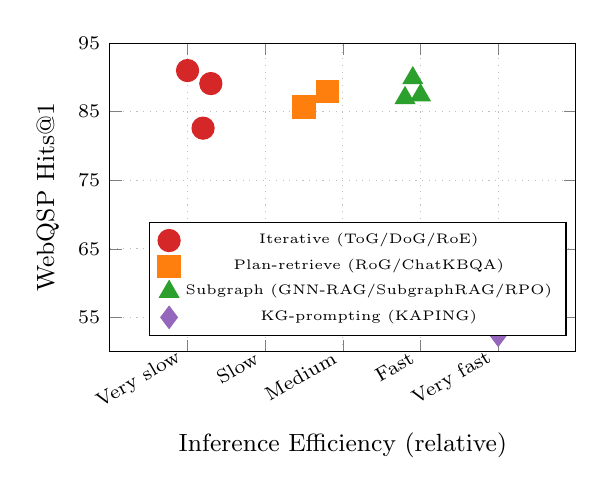
\begin{tikzpicture}
\begin{axis}[
  width=7.5cm, height=5.5cm,
  xlabel={Inference Efficiency (relative)},
  ylabel={WebQSP Hits@1},
  xmin=0, xmax=6, ymin=50, ymax=95,
  xtick={1,2,3,4,5},
  xticklabels={Very slow, Slow, Medium, Fast, Very fast},
  xticklabel style={rotate=30, anchor=east, font=\scriptsize},
  ytick={55,65,75,85,95},
  ymajorgrids=true, xmajorgrids=true,
  grid style={dotted, gray!50},
  tick label style={font=\scriptsize},
  label style={font=\small},
  legend style={font=\tiny, at={(0.98,0.05)}, anchor=south east},
]
% Iterative traversal
\addplot[only marks, mark=*, mark size=4pt, c4]
  coordinates {(1.2,82.6) (1.0,91.0) (1.3,89.1)};
\addlegendentry{Iterative (ToG/DoG/RoE)}

% Plan-then-retrieve
\addplot[only marks, mark=square*, mark size=4pt, c2]
  coordinates {(2.5,85.7) (2.8,87.9)};
\addlegendentry{Plan-retrieve (RoG/ChatKBQA)}

% Subgraph retrieval
\addplot[only marks, mark=triangle*, mark size=4pt, c3]
  coordinates {(3.8,87.0) (4.0,87.4) (3.9,89.9)};
\addlegendentry{Subgraph (GNN-RAG/SubgraphRAG/RPO)}

% KG-prompting
\addplot[only marks, mark=diamond*, mark size=4pt, c5]
  coordinates {(5.0,52.4)};
\addlegendentry{KG-prompting (KAPING)}

\end{axis}
\end{tikzpicture}
\caption{Qualitative efficiency--accuracy trade-off. Iterative methods achieve high accuracy at high LLM-call cost; subgraph retrieval methods offer a better trade-off. RPO-RAG (subgraph tier, 89.9) approaches the accuracy of DoG (91.0) at significantly lower inference cost.}
\label{fig:efficiency}
\end{figure}

\subsection{Supervision Signal Quality}

The choice of training signal critically affects retrieval quality in methods that train a retriever. Weak supervision from \emph{shortest paths} (SubgraphRAG, GNN-RAG) is easy to obtain but may not reflect the triples an LLM actually needs to answer the query—some questions require detours from the shortest path, and the LLM may reason over implicit associations that the path oracle does not encode. Plan-based supervision (RoG) is more semantically grounded but requires fine-tuning a plan generator. Reward-based supervision (RoE, RPO-RAG) directly optimizes for QA correctness and is the most task-aligned signal, though it requires a reliable reward model and is computationally intensive to train.

\subsection{KG Completeness Sensitivity}

All pre-built KG methods are sensitive to KG incompleteness: missing triples can break multi-hop chains. GNN-RAG partially mitigates this with text retrieval augmentation (RA). Methods that also retrieve relevant text passages alongside KG triples are more robust to KG sparsity. Corpus-induced KG methods face a complementary challenge: extraction errors can introduce spurious edges.

\subsection{Scalability to Large KGs}

Standard KGQA benchmarks use subsets of Freebase ($\sim$3M triples in WebQSP's neighborhood). Scaling to full Freebase (1.9B triples) or Wikidata (12B+ facts) is an open challenge. Subgraph retrieval methods with lightweight scorers (SubgraphRAG's MLP) scale better than iterative traversal methods whose LLM call count grows with beam width over a larger graph.

%% ============================================================
\section{Open Challenges}
\label{sec:challenges}

\paragraph{C1: Optimal Retrieval Supervision.}
What training signal most accurately reflects what an LLM needs from the KG? Shortest-path labels are readily available but may be noisy proxies. LLM-cited triples (triples the LLM references in its chain-of-thought) represent a stronger alignment signal but are expensive to collect at scale. An open question is whether reward-optimized methods like RPO-RAG can be made more sample-efficient.

\paragraph{C2: Relation-Awareness in Structural Encodings.}
DDE \cite{wang2025subgraphrag}, the most widely used structural feature for subgraph retrieval, aggregates neighbor distances in a relation-blind manner—all relations carry equal weight regardless of their semantic relevance to the query. Designing query-conditioned, relation-aware structural features remains an open problem, with the potential to substantially improve retrieval recall on complex multi-hop queries.

\paragraph{C3: Bridging Pre-built and Corpus-Induced KGs.}
Most methods specialize to either symbolic KGs (Freebase, Wikidata) or corpus-induced graphs (GraphRAG, HippoRAG), but real-world applications often require hybrid reasoning: domain-specific structured KGs combined with unstructured document corpora. Unified architectures that seamlessly integrate both evidence sources remain underdeveloped.

\paragraph{C4: Global vs.\ Local Query Unification.}
Corpus-level GraphRAG (community summarization) addresses global analytical queries; structured KGQA methods address local entity-centric queries. No unified method handles both well. A principled architecture that dynamically routes between local and global reasoning strategies is a significant open challenge.

\paragraph{C5: Scalability and Indexing Cost.}
LLM-based KG extraction and community summarization (MSFT GraphRAG) are expensive for large corpora. LazyGraphRAG and LightRAG reduce this cost but trade off retrieval quality. Efficient, quality-preserving indexing strategies for dynamic, large-scale corpora are needed for practical deployment.

\paragraph{C6: Evaluation Standardization.}
As discussed in \S\ref{sec:benchmarks}, the field suffers from inconsistent metrics, KG version mismatches, and reliance on gold entity linking. A standard evaluation protocol—covering end-to-end performance from raw question to answer without gold entity links—is needed to enable fair comparison.

\paragraph{C7: Generalization Across Domains and KGs.}
Most GraphRAG methods are trained and evaluated on Freebase (WebQSP, CWQ). Cross-domain and cross-KG generalization—to medical KGs, scientific literature graphs, or WikiMovies without re-training—remains largely unexplored. Methods that use the KG structure generically (e.g., via structural encodings) rather than KG-specific supervision are better positioned for transfer.

%% ============================================================
\section{Related Work}
\label{sec:related}

Several concurrent surveys cover adjacent areas. \citet{gao2023ragsurvey} and \citet{gao2024modularrag} survey the broader RAG landscape including text-based advanced RAG methods. \citet{pan2024kgllmsurvey} provide a roadmap for unifying LLMs and KGs, covering three paradigms: KG-enhanced LLMs, LLM-augmented KG construction, and synergistic methods. \citet{zhao2024ragaigc} survey RAG for multi-modal AI-generated content. Our survey is distinguished by its exclusive focus on GraphRAG, providing a finer-grained taxonomy within this subfield and the most comprehensive SOTA analysis to date.

%% ============================================================
\section{Conclusion}
\label{sec:conclusion}

We have presented a comprehensive survey of Knowledge Graph-Enhanced Retrieval-Augmented Generation, covering over 25 methods across a two-dimensional taxonomy of KG source and retrieval mechanism. Our analysis reveals a field in rapid evolution: from simple KG-prompting in 2023 to reward-optimized LLM-KG co-training in 2026. The central tension in the field is between \emph{reasoning depth} (iterative traversal, planning) and \emph{inference efficiency} (single-pass subgraph retrieval), with recent reward-based methods beginning to close the accuracy gap from the efficient end. Looking forward, the most important open problems are in supervision quality, relation-aware structural encoding, and bridging pre-built and corpus-induced KG approaches. We hope this survey serves as a structured entry point and research roadmap for this growing community.

%% ============================================================
\section*{Limitations}

This survey focuses on English-language methods and benchmarks. Multilingual and cross-lingual GraphRAG is an important direction not covered here. Additionally, due to space constraints, we do not cover KG-augmented code generation, mathematical reasoning, or multimodal QA, which are growing sub-fields where graph-structured reasoning is increasingly applied. Our SOTA tables include only a subset of results; we refer readers to the companion literature review for complete tables.

%% ============================================================
\bibliography{references}

\appendix

%% ============================================================
\section{Method Comparison Table}
\label{sec:appendix_table}

Table~\ref{tab:methods} provides a detailed comparison of all reviewed GraphRAG methods across key design dimensions.

\begin{table*}[t]
\centering
\small
\caption{Comparison of GraphRAG methods. \textit{KG Src}: Pre-built (P) or Corpus-induced (C). \textit{Retr. Unit}: retrieval granularity. \textit{Supv}: supervision signal type. \textit{LLM Use}: how the LLM is used. \textit{FT}: fine-tuning required.}
\label{tab:methods}
\setlength{\tabcolsep}{4pt}
\begin{tabular}{llllllcc}
\toprule
\textbf{Method} & \textbf{Venue} & \textbf{KG Src} & \textbf{Mechanism} & \textbf{Retr.\ Unit} & \textbf{Supv.} & \textbf{FT?} & \textbf{Multi-hop} \\
\midrule
KAPING       & ACL'23  & P & Prompt        & Triples      & None (0-shot)    & No  & Limited \\
StructGPT    & EMNLP'23 & P & Tool-call      & Structured   & None             & No  & Yes \\
ToG          & ICLR'24 & P & Traversal      & Paths        & None             & No  & Yes \\
ToG 2.0      & arXiv'25 & P & Traversal+CoT & Paths        & None             & No  & Yes \\
DoG          & AAAI'25 & P & Traversal+Debate & Paths      & None             & No  & Yes \\
RoG          & ICLR'24 & P & Plan+Retrieve  & Paths        & Relation paths   & Yes & Yes \\
ChatKBQA     & ACL'24  & P & Plan+Retrieve  & Logic forms  & S-expressions    & Yes & Yes \\
GNN-RAG      & ACL'25  & P & Subgraph       & Paths        & GNN predictions  & Yes & Yes \\
SubgraphRAG  & ICLR'25 & P & Subgraph       & Triples      & Shortest paths   & Yes & Limited \\
G-Retriever  & NeurIPS'24 & P & Subgraph (PCST) & Subgraph  & Task labels      & Yes & Yes \\
RoE          & arXiv'25 & P & RL explore    & Traces       & Answer reward    & Yes & Yes \\
RPO-RAG      & arXiv'26 & P & RL+prefer.    & Paths        & Answer reward    & Yes & Yes \\
\midrule
GraphRAG     & arXiv'24 & C & Community      & Summaries    & None             & No  & Global \\
LazyGraphRAG & Blog'25  & C & Lazy community & Summaries    & None             & No  & Global \\
HippoRAG     & NeurIPS'24 & C & PPR            & Passages     & None             & No  & Yes \\
LightRAG     & arXiv'24 & C & Dual-index     & Entities+Rel & None             & No  & Yes \\
\bottomrule
\end{tabular}
\end{table*}

\end{document}
